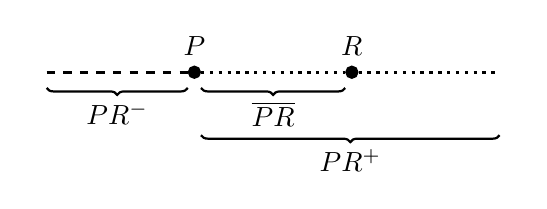
\begin{tikzpicture}
    \tikzstyle{point}=[circle,thick,draw=black,fill=black,inner sep=0pt,minimum width=4pt,minimum height=4pt]
    \node (Pleft) at (0,0) {};
    \node (P)[point,label=90:$P$] at (2,0) {};
    \node (R)[point,label=90:$R$] at (4,0) {};
    \node (Rright) at (6,0) {};
    \draw[dashed,very thick] (Pleft) -- (P);
    \draw[dotted,very thick] (P) -- (R) -- (Rright);
    \draw [thick,decoration={brace,mirror,raise=0.2cm},decorate] (Pleft) -- (P) node [pos=0.5,anchor=north,yshift=-0.25cm] {$PR^-$}; 
    \draw [thick,decoration={brace,mirror,raise=0.2cm},decorate] (P) -- (R) node [pos=0.5,anchor=north,yshift=-0.25cm] {$\overline{PR}$}; 
    \draw [thick,decoration={brace,mirror,raise=0.8cm},decorate] (P) -- (Rright) node [pos=0.5,anchor=north,yshift=-0.85cm] {$PR^+$}; 
\end{tikzpicture}
